\documentclass[11pt,oneside,a5paper]{book}
\usepackage{natbib}
\usepackage{breakcites}
\usepackage{microtype}
\usepackage[vcentering,dvips]{geometry}
\geometry{papersize={7in,9in},bottom=3pc,top=5pc,left=5pc,right=5pc,bmargin=4.5pc,footskip=18pt,headsep=25pt}
\pdfobjcompresslevel=0

\usepackage[tocindentauto]{tocstyle}
\usetocstyle{standard}
\setcounter{tocdepth}{1}
\usepackage[nottoc]{tocbibind}
\setcounter{secnumdepth}{3}

\pagestyle{headings}
\setlength{\parskip}{0.25 \baselineskip}

\usepackage{amsmath}
\usepackage{amssymb}
\usepackage{bm}

\title{\textbf{Hilbert Spaces as Generalized Conceptual Spaces} \\
in Information Dynamics of Thinking Theory}
\author{Steve Homer}
\date{}

\def\innerproduct{\langle\cdot _, \cdot\rangle}
\def\orthseq{\{ \varphi_n \}_{n=0}^\infty}

\begin{document}
\maketitle
\tableofcontents

\chapter{Conceptual Spaces}
Conceptual Spaces allow for intuitive geometric reasoning about related concepts. For instance, in the conceptual space of color with dimensions of hue, saturation, and brightness, one can reasonably make a geometric claim that “orange lies between yellow and red.”

\section{Quality Dimensions:}
Quality dimensions are the basic building blocks of a conceptual space in that they are the axes that give elements in the space meaning.  In three-dimensional Cartesian space, we refer to the xyz-axes when talking about points in the space.  By analogy, each of the xyz-axes would be a quality dimension in the 3D Cartesian space.  However, quality dimensions are more than just orthogonal unit vectors, they can also have their own specific geometry that serves to constrain the dimension. For instance, a quality dimension may have the geometry of a circle, resulting in much different behavior than the real number line.  Finally, quality dimensions allow us to talk meaningfully about similarity between objects and concepts in a space since quality dimensions contain the ideas of distance and betweenness.

\section{Integral and Separable Dimensions:}
Integral quality dimensions are ones that require one another to exist.  For instance, the hue and brightness of a color are dependent on one another. This is more than just correlation, when specifying the value of the hue, the brightness must necessarily also be specified.  Separable dimensions are ones that are independent of one another, like weight and color.  However, just because they are independent, does not mean they can't be correlated.

\section{Domains and Conceptual Spaces:}
A domain is a set of integral dimensions that are separable from all other dimensions.  In a sense, it is the minimum description needed for a given space.  Often, different domains will be correlated to one another, and combining them together yields a full-fledged conceptual space.

\section{Similarity, Distance, Betweenness:}
Humans have an innate sense of similarity without being able to fully describe why two things are similar.  It seems obvious that a rectangle is more similar to a square than a circle, but we're able to intuitively spy similarity in very abstract realms.  For instance, most people would naturally agree that country music is closer to rock than it is to classical, but would be hard-pressed to give an exact definition or method of why this is so.

Conceptual spaces allow this innate sense of similarity to be codified in the intuition of geometry, betweenness, and distance.  Given a betweenness relation for a conceptual space, one can say that a given object is between two other objects, which allows us to say that one is closer to another than the third.  In our case, we will study conceptual spaces equipped with a distance measure.  This allows us to examine the distance between ideas, saying that one is closer to another.  Proximity here serves as our measure of similarity.

\section{Convexity of Properties and Concepts:}
Gardenfors says that a property or concept is a convex region in a given conceptual space.

\section{Higher-order conceptual spaces}
Generated from the combination of lower-order QDs according to a pattern
i.e. A transform from lower to higher abstraction

Higher-order conceptual spaces are simply combinations and transformations of lower-order conceptual spaces.  This often comes with a dimensionality reduction, thought not necessarily; however, the higher-order nature of the spaces always means that it is more abstract than the spaces it is generated from.

This is to distinguish it from combinations that serve to more tightly specify a space.  For instance, given the color space over the space of human phenotypes, overlaying the two results in a restricted color space of human skin tones, not a more abstract space.  (Is this actually NOT higher-order?)  



\chapter{Hilbert Spaces}

\begin{quote}
  "Hilbert spaces are the means by which the ordinary experience of Euclidian concepts can be extended meaningfully into the idealized constructions of more complex math."
\end{quote}

\section{Motivation}

Since we need to represent oscillations in a conceptual space, we need a more general notion of what a space is than a finite-dimensional Euclidian space.  The generalization employed here is that of Hilbert spaces, most famously used in quantum mechanics to model wave functions.

Hilbert spaces are characterized by their inner product $\innerproduct$, which can be used to generate an infinite orthonormal sequence $\orthseq$.  Similar to dimensions $(\hat{x}, \hat{y}, \hat{z})$ that characterize three dimensions in Cartesian space, each element in the orthonormal sequence is normalized and orthogonal to each other element, and therefore can be thought of as a dimension. 

Since any function in a Hilbert space can be represented by its Fourier series over an orthonormal sequence, not only can we represent any function, but by employing a different inner product, we generate a different orthonormal sequence and therefore a different representation of that same function. This allows us to have different perspectives of the same "raw" data.  This is analogous to how the coordinates $(1,1)$ representing $(x,y)$ in a 2-dimensional Cartesian space have a different meaning than the coordinates $(1,1)$ representing $(r, \theta)$ in a 2-dimensional radial space.

\section{Complete Inner Product Space}
\begin{itemize}
  \item \textbf{Vector Space:} Dimensions and rules for combining vectors
  \item \textbf{Norm $\|.\|$:} Measure of the size of a vector
  \item \textbf{Inner Product $\innerproduct$:} Defines orthogonality, projections, and angles of vectors
  \item \textbf{Completeness:} Space is big enough to include norm of converging sequences
\end{itemize}

The induced norm $||.||$ is defined in terms of the inner product $\innerproduct$:
\begin{equation}
  \|f\| = \langle f, f \rangle^{1/2} 
\end{equation}
but only if the Cauchy-Schwarz (triangle) inequality holds:
\begin{equation}
|\langle f, g \rangle| \leq \|f\|\|g\| 
\end{equation}

\section{Gram-Schmidt Orthogonalization}
Given an inner product $\innerproduct$ for Hilbert space $\mathcal{H}$, one can generate a complete orthonormal sequence by performing the following procedure:

Find $\{ \varphi_n \}_{n=0}^{N-1} \in \mathcal{H}$ given $\{ f_n \}_{n=0}^{N-1} \in \mathcal{H}$ independent vectors
\begin{equation}
\begin{gathered}
  \varphi_0 \overset{\bigtriangleup}{=} \frac{f_0}{\| f_0 \|} , \quad
  \nu_n \overset{\bigtriangleup}{=} f_n - \sum_{m=0}^{n-1} \langle f_n , \varphi_m \rangle , \quad
  \varphi_n \overset{\bigtriangleup}{=} \frac{\nu_n}{\| \nu_n \|}
\end{gathered}
\end{equation}

Essentially, at each step n, remove all lower $\varphi_n$ projections from the current function $f$ and normalize it.  By removing all projections on lower $\varphi_n$ at each step, we ensure that what results is orthogonal to everything below it. 

\section{Representing Oscillations}

Functions can be thought of as point or vector in a given Hilbert Space characterized by its inner product $\innerproduct$. Since an oscillation is just a periodic function, we can represent any oscillation to full precision as a point in a Hilbert space.  Specifically, any given function $f$ can be decomposed into its Fourier series:

\begin{equation}
  f = \sum_{n=0}^\infty \langle f, \varphi_n \rangle \varphi_n
\end{equation}

Since each $\varphi_n$ represents an orthonormal basis vector, this decomposition allows us to represent any oscillation by an infinite vector, where each dimension of the vector corresponds to a $\varphi_n$.



\chapter{Information Theory}

\section{Motivation}

\section{Entropy}

\section{Information Content}

\section{N-Gram Models}

\chapter{Inductive Constraints}
Multiple levels of abstraction constrain one another

Major references:
The acquisition of Inductive Constraints (Kemp),
The Discovery of Structural Form (Kemp, Tenenbaum),
Hierarchical Bayesian Models and Hierarchical Markov Models

\chapter{Information Dynamics of Thinking}

\section{What it do?}

\section{Sequential Memory}
The sequential memory in IDyOT is represented as a hierarchy of chains of symbols. As the agent perceives a continuous stream of perception from the environment, it first discretizes that stream into moments, and links those discretized percepts as symbols in an ever-growing chain.  By examining time-varying information-theoretic properties of this chain, it can be chunked into a series of segments composed of a sequence of symbols.  This segment can then be abstracted by a representative symbol in the superior layer and can be said to subsume the inferior segment.  This process is done recursively until no more abstraction can be performed.

\section{Semantic Memory}
If the sequential memory can be though of as how concepts relate to eachother over time, semantic memory can be thought of as how those concepts relate to eachother outside of time.  In IDyOT this is modeled using conceptual spaces.  At any given layer of abstraction in the sequential memory, there is a "parallel" semantic space for the symbols of that layer.  This allow us to think of a segment of symbols in sequential memory as a trajectory of concepts in semantic memory.  By looking at a spectral representation of this trajectory, the time-varying properties of the segment are removed, and this spectral representation can be thought of as an abstraction of the segment, and therefore as the abstracted symbol in the superior layer of the sequential memory.

\section{Categorization}
\label{section:categorization}

Beyond the necessity for categorization due to the problem of content sparsity (see section \ref{section:content-sparsity}), categorization of representations is necessary to model the properties and concepts determined by regions of conceptual spaces (see section \ref{section:convexity-properties-concepts}).  Since we cannot \textit{a priori} know the bounds of the regions of concepts in a conceptual space, we instead build them up through categorization, discussed here.

\subsection{Information Content Reduction Criterion} 
\label{section:information-content-reduction-criterion}

Since the goal of an IDyOT is to be as information-efficient as possible in its representation of concepts, the primary way to do this is categorize two different symbols together if they lead to an overall reduction in information content of the space.  However, if this reduction by information content measure was the only method used to determine categories, there would be nothing to stop all symbols from being categorized together.  If all the symbols are the same, the information content is maximally reduced, but the result is a meaningless stream of monotony.  Obviously, this is unrealistic and undesirable.

\subsection{Categorical Convexity Criterion}
\label{section:categorical-convexity-criterion}

To push back against the reduction by information content is the categorical convexity criterion.  In section \ref{section:convexity-properties-concepts}, we saw that categories correspond to convex regions in a conceptual space.  In Hilbert spaces, categories would then translate to an infinite-dimensional hyperellipsoids.  In IDyOT, the convexity criterion guarantees that for any two symbols in a given category, there is no symbol from a different category between those two symbols.

Though this criterion is simple in formulation, the definition of what \textit{between} actually means can vary depending on the space in question.  Even when the space is unidimensional, the definition of \textit{between} is somewhat arbitrary.  For instance, take a space that is wrapped around a circle.  Any point is between any other two points, depending on which direction around the circle you move.  Things get even less clear when moving into higher dimensions, where oftentimes, even a partial natural ordering is impossible.

Therefore, instead of looking at betweenness at all, we incrementally build up categories by way of an inclusion radius $\rho$ around each point \citep{wiggins2019learning}.  If another point falls within the inclusion radius of a category, that point is grouped into that category.  In this way, we can ensure that there is never an interloper in a category, since if it was intruding on the region of the category, it would already be a member.

\subsection{Adaptive Categories}
\label{section:adaptive-categories}

Since we utilize an inclusion radius to determine the categorization candidates for a new point, this would naively result in a partition of the space in which all categories are the same size, since they all use the same radius.  However, the categories of a given conceptual space are likely to be variable in size, and therefore we require a mechanism to adapt the size of a category according to the observations as they are added to the space.

In order to ensure this adaptability, we maintain a mean $\mu$ and variance $\sigma^2$ of a multidimensional Gaussian prior distribution $\mathcal{N}(\mu,\sigma^2)$ for each category.  Whenever a new point $x$ is added to the category $c$, we perform a posterior update, which becomes the new prior of the category in future categorization.  In using a Gaussian prior, the centroid of the category corresponds to the prior mean, whereas the radius of the category corresponds to the $\|3\sigma\|$ (or 99.7\% of the volume of the Gaussian) which can be found from the prior variance $\sigma^2$.

As more instances are added to a category, its mean will converge to a more somewhat stationary mean, and its variance will tend to decrease, corresponding to a reduction in the radius, though this will happen less if the constituent points of a category are spread out.  This makes the size of the category adaptive to its observed members and allows different categories to have different volumes.  By using the spherical Gaussian prior, the boundary-convexity of each category is ensured.

Since points are being added to the space incrementally, the posterior update of the category is also performed incrementally \citep{murphy2007conjugate} by maintaining not only the prior mean and variance, but also sample mean and variance for each category.  Therefore, whenever a new point $x_t$ is added to a category, the moments of the distribution are updated as follows:

\begin{align}
\label{equation:gaussian-posterior-update}
  m_t &= m_{t-1} + \frac{x_t - m_{t-1}}{n_t}
    \tag*{(Sample Mean)} \\
  s_t^2 &= s_{t-1}^2 + \frac{(x - m_t)(x - m_{t-1}) - s_{t-1}^2}{n_t}
    \tag*{(Sample Variance)} \\
    \mu_t &= \frac{\mu_{t-1} s_t^2 + x \sigma_{t-1}^2}{\sigma_{t-1}^2 + s_t^2}
    \tag*{(Posterior Mean)} \\
    \sigma_t^2 &= \frac{\sigma_{t-1}^2 s_t^2}{\sigma_{t-1}^2 + s_t^2}
    \tag*{(Posterior Variance)}
\end{align}

\subsection{Maximum Information Content Reduction}
\label{section:maximum-information-content-reduction}

When a new point is added to the space, there may be multiple candidate categories for which the point falls within their inclusion radius.  When this happens, the heuristic of maximum information content reduction is employed.  Put simply, the new point is grouped with the category with the highest information content, as including the point in that category results in the largest reduction in information content out of the candidates.  Unfortunately, this results in a violation of the categorical convexity criterion due to the restriction in this implementation that each point must belong to exactly one category.

Instead, the union of all candidate categories for the point could be combined to create a single category representing all the points of the constituent categories.  This has the benefit of both greatly reducing information content while still maintaining categorical convexity.  However, in practice, there is enough incidental overlap between what should be distinct categories that a large amount of points get categorized together which should not be, resulting in a small number of large, but meaningless groupings.  This union categorization scheme is a likely avenue of future research.

\section{Segmentation}

Segmentation is the process of dividing an input stream into discrete chunks according to a difference function.

\subsection{Difference Function}
The difference function operates on the stream of symbols entering a given dimension and decides where segments begin and end.  Though there are a variety of ways in which to determine where to cut in this chain of symbols, here we will look at their information-theoretic properties to determine a meaningful cut. Primarily, we will look at moving entropy of the signal.  If the entropy rises, then a cut should be a made, marking the end of the current segment and the beginning of a new one.

Since entropy represents the amount of uncertainty at what comes next, it makes sense that a jump in entropy would mark the beginning of a new segment.  For instance, at the beginning of a sentence, entropy is high because the listener has little idea what the speaker will say next. As the sentence proceeds, the speaker will be better able to predict what comes next, meaning entropy is decreasing until the end of the sentences.  Once the sentence is finished, the listener again is less sure what will come next, and so entropy rises.  Therefore, at this rise in entropy, we would make a cut, resulting in a segment naturally representing the sentence just spoken.

This segmentation process results in two problems stemming from the two types of sparsity inherent in the segmentation and subsequent abstraction.

\subsection{Symbol Sparsity}
The first kind of sparsity arises from the length of the segment produced in the segmentation process.  Since the abstraction of the segment is its spectral transform, and we use the Discrete Fourier Transform (see section ?) to find the representative symbol in the superior abstraction layer, we run into precision problems due to the uncertainty principle of signal sparsity.  When performing a DFT, the signal precision is limited by the number of non-zero coefficients in either the time or frequency domain.  Therefore, if the number of symbols in a given segment is small, its spectral representation will be imprecise.  Therefore, it is necessary to perform interpolation (see section ?) to fill out the signal, so that high precision is maintained in the spectral transformation.

\subsection{Content Sparsity}
The second kind of sparsity is due to the nature of the symbol contents.  Since in the case of audio perception, the content of a symbol is a high-dimensional tensor of complex coefficients, not only are the possible values of each dimension uncountably infinite, there are a high number of uncountably infinite dimensions for each symbol.  Therefore, it is incredibly unlikely that any two symbols have exactly the same value for every dimension in the conceptual space in which they live.  

This poses a problem for determining the entropy and information content of symbols, which rely on the probability of a symbol.  If every symbol is unique, in the limit, the probability of seeing one in the signal is 0, meaning the entropy and information content each symbol in the signal would be 0. Really, the the probability of a unique event is meaningless, and therefore, even talking about its entropy is also meaningless.  

Though the space in which the symbols live is so sparse, we would still like to say that if two symbols are close enough together, for all intents and purposes (intensive porpoises), they are the same symbol.  This is accomplished through categorization (see section ?), where a label is attached to each symbol according to its category.  If two symbols have the same label, then they are equal, even though they may have different contents, that is, different values in their complex tensors.

\subsection{Symbol Generation}
When a segment is cut from the stream of symbols in a given dimension, a new symbol is generated that represents that segment in the superior abstraction layer.  At least in the case of all dimensions supervenient on audio perception, this means that the abstracted symbol is the spectral transformation of the segment.

\section{Interpolation}
When talking about trajectories through conceptual spaces, we refer to interpolation as the use of virtual concepts that factor into the abstraction to the superior space.  Since we formalized conceptual spaces as Hilbert spaces, we can analogously talk about drawing a curve or curve through points in the space.  Hence, the process of interpolation is simply sampling from a regression.

\subsection{Symbol Sparsity}
As discussed in section (?) on segmentation, interpolation is necessary to deal with symbol sparsity in a given segment.  To reiterate, this problem arises due to the use of the Discrete Fourier Transform in the abstraction process.  Since the precision of a signal, either in the time or frequency domains, is determined by the number of non-zero coefficients describing that signal, if the segmentation process results in a relatively short segment, the number of coefficients will be small, and the resulting transformation imprecise.

The way to deal with this imprecision is fill in coefficients in an informed way such that the transform of the signal accurately represents the original signal while maintaining higher precision.  This is valid because we can think of the sparse signal as a sequence of samples from a function, and by intelligently regressing on those samples, we can obtain the representative function.  By interpolating, we are simply drawing more samples from that regressed function to deal with the precision limits of the DFT.

\subsection{Spatial Geometry}
Though interpolation is necessary primarily to deal with symbol sparsity of a segment, it is also the main vehicle in which the geometry of the conceptual space induces the path of the trajectory of symbols.  Since in the Information Dynamics of Thinking, the interpretation of any space is determined by its inner product, we need to interpolate through that space in order to "see" the geometry.

\begin{figure}
  \centering
  \begin{subfigure}[H]{0.45\linewidth}
    \def\svgwidth{\linewidth}
    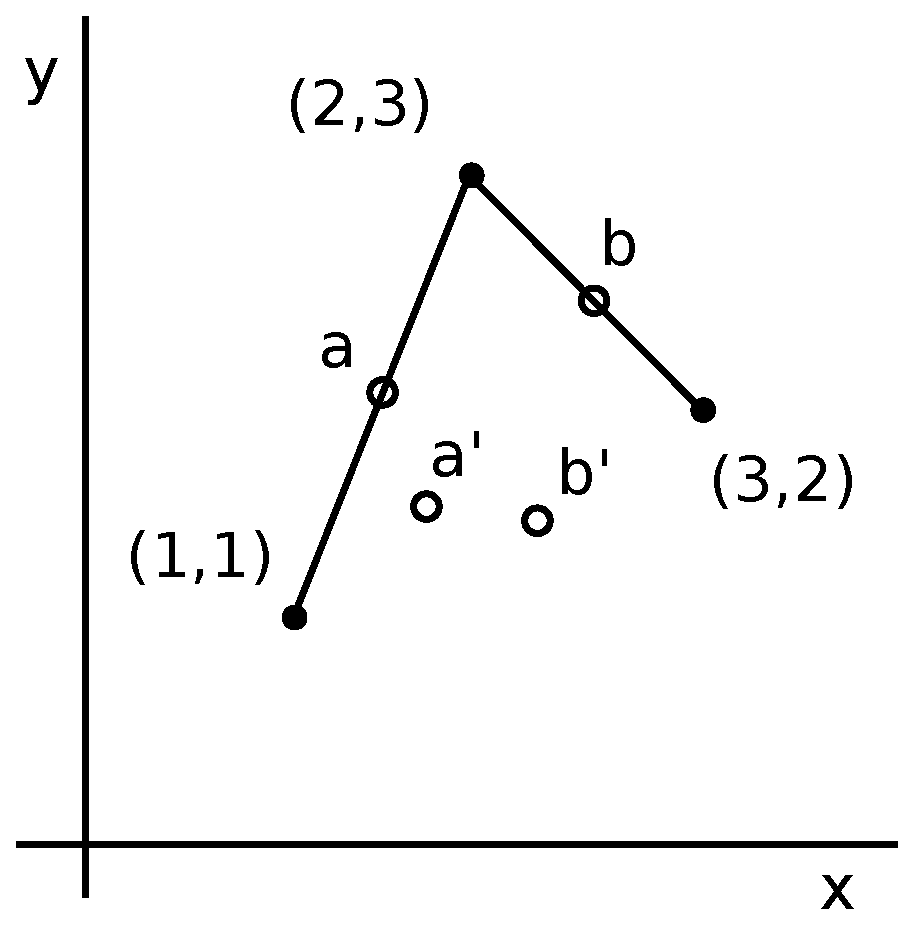
\includegraphics[width=\linewidth]{fig/interpolation-cartesian.eps}
    \caption{Cartesian Trajectory}
  \end{subfigure}
  \begin{subfigure}[H]{0.45\linewidth}
    \def\svgwidth{\linewidth}
    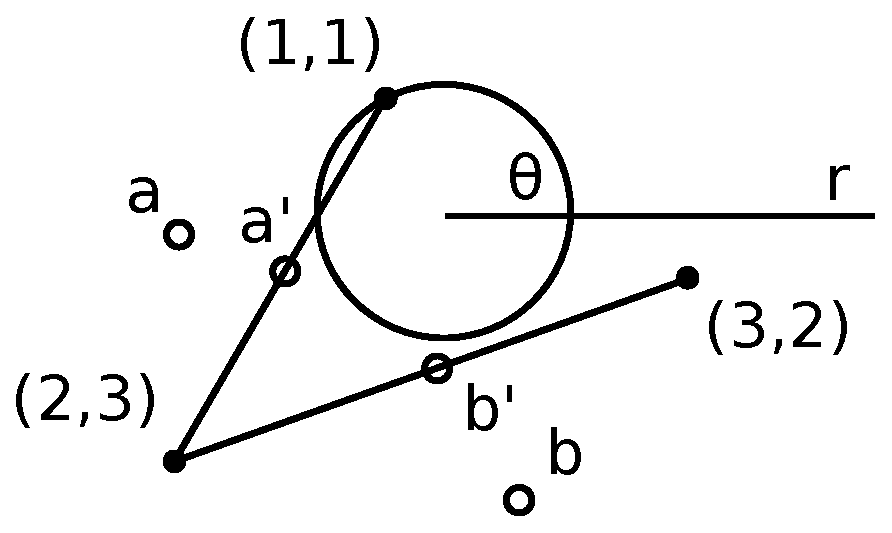
\includegraphics[width=\linewidth]{fig/interpolation-radial.eps}
    \caption{Radial Trajectory}
  \end{subfigure}
  \caption{Example of effect of spatial geometry on interpolation}
\end{figure}

For instance, suppose we have three 2D symbols of which we want to draw a trajectory through. Consider two different spaces for conceiving those points: Cartesian (x, y) and Radial (r, $\theta$). Suppose we take the DFT of three points, i.e. as a trajectory without interpolation, in each of the two spaces.  Since the values of each point are exactly the same for both spaces, when examining the transform, there would be no way to tell which space it came from.  If instead we draw lines through the points and interpolate before taking the transform, we see clearly that the interpolated points differ between the two spaces, and so the transform of each trajectory will also be different.  In this way, the information about the geometry of the space can have an effect on the abstraction of the trajectory in that space.

\subsection{Types}
Since our conceptual spaces are represented as Hilbert spaces, interpolating a trajectory through a sequence of concepts is equivalent to regressing through the points of the space and sampling from that regression.  As such, we can employ any number of regression techniques from the literature to determine an appropriate trajectory.

\subsubsection{Connect the Dots}
Though not really regression per say, the simplest method for interpolating between points would be to just draw a straight line between them and sample from that line.  This method has the benefit of being very simple, and may prove to be near-equivalent to other methods if the number of interpolated points is low enough.

The problem with this method is that it is not continuously differentiable and therefore quite "sharp".  This would manifest in the DFT by resulting in high amplitudes at higher frequencies.  It is difficult to say a priori if this is desirable, but it seems in general that we would prefer smoother functions through these points to avoid this effects.

\subsubsection{Gaussian Regression (Kriging)}
One method for creating a smooth curve through these points is Gaussian Regression.  By thinking of the sequence of points as a multivariate Gaussian distribution, we can think of a distribution of trajectories or functions, i.e. a process, through these points.  By finding the mean function of this process we can find the maximum a posteriori trajectory of the process, resulting in the highest likelihood function through a sequence of points.  This method automatically avoids problems of overfitting inherent in higher-order transformation linear regression methods, though has the problem being computationally expensive.

By utilizing the square exponential kernel for Gaussian regression, the resulting curve will not only by the MAP curve, but also infinitely differentiable, meaning that it is hella smooth.  This smoothness results in a reduction of large high frequency amplitudes that could potentially happen in simpler methods like Connect-the-dots.


\chapter{Abstraction}

When a segment is produced in the segmentation process, it is abstracted to a single symbol in the superior abstraction layer.  Since each dimension is composed of both an alphabet of symbols and a conceptual space in which those symbols live, a segment of symbols can be though of as a trajectory through a conceptual space.  Viewing this trajectory as a sequence of points in a high-dimensional space, one can abstract out the time variant properties of the signal by viewing it in terms of its spectral properties.  When viewed spectrally, this same trajectory can be thought of as a single point, creating a mapping from the segment in the inferior dimension to the a point in the superior abstraction layer.

\section{Fourier Transform}
In the Information Dynamics of Thinking, the Fourier Transform is used to take the time-domain trajectory of the inferior layer to the frequency-domain point of the superior layer.  Though there are other spectral representations of a signal available besides the Fourier transform, there is evidence, especially in the auditory domain, that the brain operates on frequency transformations of time-varying signals (organ of corti), and so it is employed here.

Since the segment is a trajectory of discrete points in a Hilbert space, we use the discrete fourier transform to take the trajectory from time-domain to frequency-domain.  It is important to note that the (discrete) Fourier transform is a linear operator on the Hilbert space, meaning essentially that the \textit{shape} of the signal does not change in the tranformation, only its domain.  Therefore, use the independence of the frequency bins resultant from the DFT to represent those bins as dimensions in the superior abstraction layer.

\section{Tensor Rank Promotion}
To clarify this point, consider figure (below).  When the time-varying sound signal is transduced at the base perceptual level, it can be represented as a row vector of real values, where each element in the row represents the signal amplitude dimension at that time step. This sounds signal is of finite length, and can be thought of as a moving window of attention. Since it is a linear operator, performing the DFT on this signal results in a row vector of the same length, only now with complex elements in the frequency domain.  Since each element of this row vector represents an orthonormal frequency bin, we can alternatively think of this row vector as a column vector, where each row in the column represents a different dimension.  This transposition of row vector to column vector is what takes the frequency-domain trajectory to a single point in its dual space.

Now, when we have a trajectory of in this frequency space, instead of operating on a row of real values as in the sound signal, we are operating on a row of complex column vectors, and the trajectory now looks like a matrix.  Taking the DFT of this trajectory and transposing it to be represented as a point, the abstracted point is now a matrix.  Taking a trajectory of these matrices results in a point represented by a cube (3d rectangle?).  Taking a trajectory of these cubes results in a point represented by a hypercube, and so on.

Therefore, when moving from one abstraction layer to its superior, the complex tensor representing the contents of the symbol increases in rank, which is what is meant by tensor rank promotion.

(Figure of tensor rank promotion)

\section{Component-wise Fourier Transform}
When performing the Fourier transform on a tensor of any rank, it should be noted that each component in the tensor is independent from every other component.  Though this is not necessarily true in general, due to the particular hierarchical construction of these spaces, each component is decoupled from the rest.  Starting at the bottom, the time-domain sound signal is transformed into a frequency-domain signal of coefficients in independent frequency bins.  It is this independence that allowed us to represent it as a point with those frequency bins as dimensions.  Performing the DFT on the trajectory of column vectors results in independent frequency bins filled with column vectors with independent entries, meaning all components are independent one another.

Recursively performing the DFT on tensors with independent components results in higher rank tesnors with independent components.  This component-independence of the tensor means that the DFT should be taken component-wise, since all other cross-component terms would involve orthgonal components, resulting in zero terms.

\include{tex/tensors}
\include{tex/inner-products}

\end{document}
